\documentclass[conference]{IEEEtran}
\IEEEoverridecommandlockouts
\usepackage[T1]{fontenc}
\usepackage{newtxtext,newtxmath}
\usepackage{graphicx,booktabs,multirow,array,xcolor,microtype,tikz}
\usepackage[hidelinks]{hyperref}
\usepackage{cite}
\usetikzlibrary{positioning,fit,arrows.meta,backgrounds,calc}

\definecolor{ink}{HTML}{1F2933}
\definecolor{muted}{HTML}{7B8794}
\definecolor{lang}{HTML}{2563EB}
\definecolor{vis}{HTML}{059669}
\definecolor{act}{HTML}{D97706}
\definecolor{pass}{HTML}{047857}
\definecolor{fail}{HTML}{B91C1C}
\newcommand{\pass}{\textcolor{pass}{\textbf{pass}}}
\newcommand{\fail}{\textcolor{fail}{\textbf{fail}}}
\newcommand{\h}[1]{\textbf{H#1}}
\setlength{\tabcolsep}{3.2pt}
\raggedbottom

\begin{document}
\title{How Small Can VLA-JEPA Get? Post-Training\\ Compression of a Robot Policy on LIBERO}
\author{\IEEEauthorblockN{Noah Sprenger \qquad Fernando Nogueira}
\IEEEauthorblockA{CSI 5341, University of Ottawa \quad Code: \url{https://github.com/seofernando25/csi5341-vla-jepa}}}
\maketitle

\begin{abstract}
VLA-JEPA couples a 2B-parameter vision--language model with a flow-matching action head and reaches 95\% success on LIBERO-Spatial, with a measured peak of 5.6\,GB allocated GPU memory at batch size one. We test whether post-training compression keeps that success on this suite. Quantizing only the language-decoder linear layers to NF4 cuts peak memory by 36.9\% with a paired success change of $+0.8$ points (95\% CI $-0.6$ to $+2.2$, 500 trials). LLM.int8 cuts 23.3\% and misses our 25\% target, which equals the ideal INT8 saving for the decoder weights. A sweep of 201 compression recipes finds that the language decoder is the precision bottleneck, while vision and action weights survive 2-bit quantization. Four joint recipes keep 93.4--98.0\% success at 0.94--1.51\,GB (73--83\% less memory). Two (C1, C2) use a vocabulary restricted to the test prompts, so we flag them and draw no conclusion from them; C3 and C4 use neither that nor any calibration data. Under the stock execution path every compressed policy is 1.2--2.0$\times$ slower, because that path is launch-bound. A CUDA-graph engine speeds up B16 itself from 77.5 to 28.5\,ms; the data-free NF4 policy C4 then runs at 31.6\,ms in 1.51\,GB with 98.0\% success. Offline action divergence on fixed frames predicts gross failure ($\rho=-0.67$, 163 recipes) but cannot rank near-lossless ones. Replacing the backbone with SmolVLM2-500M failed (2.2\%).
\end{abstract}

\section{Introduction}
Vision--language--action (VLA) policies map camera images and an instruction to robot actions~\cite{openvla,pi0}. VLA-JEPA~\cite{vlajepa} adds a V-JEPA~2 latent world model~\cite{vjepa2} during training to a Qwen3-VL-2B backbone~\cite{qwen3vl} and a flow-matching action head. Its weights alone occupy 5.5\,GB in BF16, which excludes many embedded GPUs. We ask how far the \emph{trained} policy can be compressed without retraining, and what breaks first.

Our proposal stated one hypothesis. The feedback asked for justified thresholds and more depth, so we test four:
\begin{itemize}
\item[\h1] Quantizing the language-decoder linear layers reduces peak inference memory by $\geq$25\% and lowers LIBERO-Spatial success by $\leq$5 points.
\item[\h2] Tolerance to compression differs by module: the language decoder is more sensitive than the vision encoder or action head.
\item[\h3] At batch size one, lower memory does not imply lower latency.
\item[\h4] The change in predicted actions on fixed observations predicts closed-loop failure, so it can screen recipes without rollouts.
\end{itemize}

\textbf{Thresholds.} The 25\% memory target is the ideal saving of 8-bit decoder weights: 1.41B linear parameters lose one byte each, 1.41\,GB of a 5.61\,GB peak, or 25.1\% (Fig.~\ref{fig:budget}). \h1 therefore asks whether runtime overhead consumes the theoretical saving. The 5-point bound allows the 5\% baseline failure rate to at most double. With 500 paired trials, the 95\% interval on a paired difference spans 2--4 points, narrow enough to separate a 5-point drop from no change.

\textbf{Contributions.} (i) A matched 500-trial evaluation of INT8 and NF4 decoder quantization with paired statistics. (ii) A module-level sensitivity map over 201 recipes and 21 component domains. (iii) Three deployable recipes below 1.4\,GB with reserved-trial confirmation. (iv) A failure analysis linking offline action change to task success.

\begin{table*}[t]
\centering\small
\caption{Experimental design. All rows share the checkpoint, task suite, states, seeds, action horizon, GPU and software versions; E7 also changes the flow steps.}
\label{tab:design}
\begin{tabular}{@{}l>{\raggedright}p{3.3cm}>{\raggedright}p{3.6cm}>{\raggedright}p{3.8cm}>{\raggedright\arraybackslash}p{4.6cm}@{}}
\toprule
ID & Question & Varied & Sample & Analysis and decision rule \\
\midrule
E1 (\h1) & Does decoder quantization keep success? & Decoder linear precision: BF16, INT8, NF4 & 500 reserved rollouts per arm & Paired bootstrap; pass if memory reduction $\geq$25\% and $\Delta\geq-5$ pp \\
E2 (\h2) & Which modules tolerate compression? & Module $\times$ method $\times$ strength; 201 recipes & 80 fixed frames; 10-trial smoke (163); 100-trial development (24) & Development gate $\geq$77/100 (B16 82 $-$5); selection frozen before E3 \\
E3 & Do joint recipes hold on reserved trials? & Three frozen joint recipes & 500 reserved rollouts each & Wilson and paired intervals; report regardless of outcome \\
E4 (\h3) & Does lower memory mean faster? & All E1/E3 arms & $3\times500$ timed predictions & Median and p95 latency vs.\ peak memory \\
E5 (\h4) & Where and why do arms fail? & --- & Per-episode outcomes; 80-frame action change & Paired transitions per task; Spearman $\rho$ \\
E6 & Can a smaller backbone replace Qwen? & SmolVLM2-500M + adapter, 10k fine-tuning steps & 500 reserved rollouts & Same as E1 \\
E7 (\h3) & Is the slowdown intrinsic to quantization? & Execution engine (stock or CUDA graph), flow steps (4 or 1), dense or packed NF4 weights & $3\times500$ timed predictions per variant; 500 reserved rollouts for C4 & Same as E1; the one-step setting comes from the E2 smoke screen \\
\bottomrule
\end{tabular}
\end{table*}

\section{Related Work}
\textbf{VLA policies.} OpenVLA~\cite{openvla} discretizes actions from a 7B language model; $\pi_0$~\cite{pi0} and VLA-JEPA use flow matching. SmolVLA~\cite{smolvla} trains a 0.45B policy from scratch on a SmolVLM backbone~\cite{smolvlm}. We compress an existing policy instead of training a small one.

\textbf{Quantization.} LLM.int8~\cite{llmint8} keeps outlier features in FP16; NF4~\cite{qlora} stores 4-bit normal-float weights with double-quantized scales. GPTQ~\cite{gptq} and AWQ~\cite{awq} calibrate weights on sample inputs; HQQ~\cite{hqq} quantizes without calibration down to 2 bits. QuantVLA~\cite{quantvla} adapts post-training quantization to VLA action experts.

\textbf{Pruning.} Wanda~\cite{wanda} and SparseGPT~\cite{sparsegpt} prune individual weights; structured pruning removes channels, heads or layers, and EcoVLA~\cite{ecovla} applies it to VLAs. We rank layers by linear CKA~\cite{cka} between block input and output. Unstructured masks save no memory without sparse kernels, so we report memory only for structured and packed formats.

\section{Method}
\begin{figure}[t]
\centering
\resizebox{\columnwidth}{!}{%
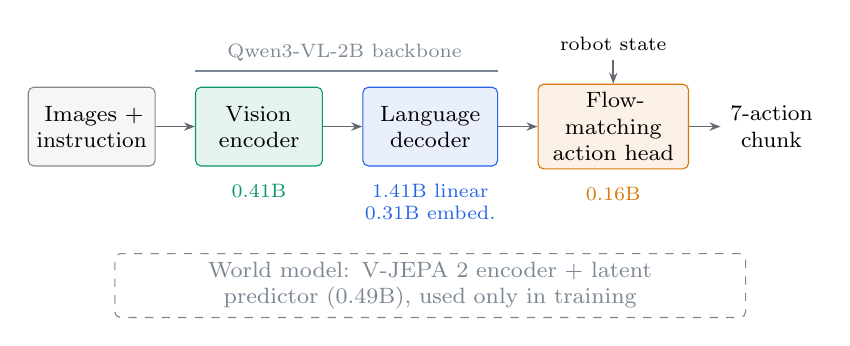
\begin{tikzpicture}[
  font=\footnotesize, node distance=4mm and 5mm,
  box/.style={draw=ink!55, rounded corners=2pt, fill=ink!4, align=center, minimum height=10mm, inner sep=3pt},
  tag/.style={font=\scriptsize, align=center},
  arr/.style={-{Stealth[length=4pt]}, draw=ink!70, line width=.6pt}]
\node[box, text width=14mm] (in) {Images +\\instruction};
\node[box, right=of in, text width=14mm, draw=vis, fill=vis!10] (vis) {Vision\\encoder};
\node[box, right=of vis, text width=15mm, draw=lang, fill=lang!10] (lm) {Language\\decoder};
\node[box, right=of lm, text width=17mm, draw=act, fill=act!10] (act) {Flow-matching\\action head};
\node[right=4mm of act, align=center] (out) {7-action\\chunk};
\draw[arr] (in) -- (vis); \draw[arr] (vis) -- (lm); \draw[arr] (lm) -- (act); \draw[arr] (act) -- (out);
\node[tag, below=1mm of vis, text=vis] {0.41B};
\node[tag, below=1mm of lm, text=lang] {1.41B linear\\0.31B embed.};
\node[tag, below=1mm of act, text=act] {0.16B};
\node[tag, above=3mm of act] (st) {robot state}; \draw[arr] (st) -- (act);
\draw[muted, line width=.5pt] ($(vis.north west)+(0,2mm)$) -- ($(lm.north east)+(0,2mm)$);
\node[tag, text=muted, above] at ($(vis.north)!0.5!(lm.north)+(0,2mm)$) {Qwen3-VL-2B backbone};
\node[box, dashed, fill=white, draw=muted, text=muted, minimum height=6mm,
  below=11mm of lm, text width=78mm]
  (wm) {World model: V-JEPA 2 encoder + latent predictor (0.49B), used only in training};
\end{tikzpicture}}%
\caption{VLA-JEPA inference path with parameter counts. Colored modules are the compression targets; mergers connect vision features to the decoder. The world model is loaded by default but unused at inference.}
\label{fig:arch}
\end{figure}

\textbf{Policy.} We use the released LIBERO checkpoint of the LeRobot port~\cite{lerobot} (\texttt{VLA-JEPA-LIBERO}), pinned by revision (Fig.~\ref{fig:arch}). The policy predicts seven actions with four Euler flow steps and executes all seven before replanning. Nothing in this report retrains Qwen.

\textbf{Compression arms.} \emph{Study A} quantizes every \texttt{nn.Linear} in the 28-layer Qwen decoder after the checkpoint loads: Q8 with LLM.int8 (outlier threshold 6) and Q4 with NF4 (double quantization, BF16 compute). Every other module stays BF16. \emph{Study B} applies 201 recipes to individual modules and joint deployments: bitsandbytes INT8/NF4, HQQ 2--4 bit, GPTQ, AWQ-style scaling, TorchAO W8A8, magnitude/Wanda/SparseGPT sparsity, and structured removal of MLP channels, attention heads, layers and tokens. Calibrated methods use 20 development frames; no recipe sees reserved trials. Joint deployments also drop the unused world model and may restrict the vocabulary to the 53 token IDs that LIBERO instructions use.

\begin{figure}[t]
\centering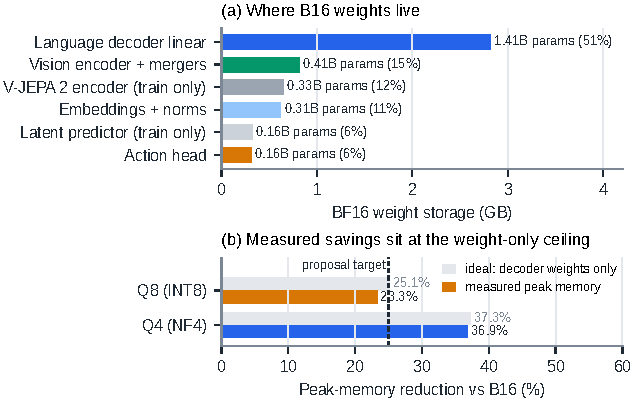
\includegraphics[width=\columnwidth]{figures/budget.pdf}
\caption{(a) B16 parameters by module. (b) Weight-only savings ceiling for quantizing the decoder linear layers versus the measured peak-memory reduction.}
\label{fig:budget}
\end{figure}

\textbf{Protocol.} Table~\ref{tab:design} lists the experiments. All runs use one RTX~3090, PyTorch 2.11, Transformers 5.5.4 and bitsandbytes 0.50.2. Rollouts use the ten LIBERO-Spatial tasks~\cite{libero} and the 50 official initial states per task, with fixed per-episode seeds and a 280-step limit. Development trials use 10 different states per task, disjoint by hash. Success intervals are Wilson intervals~\cite{wilson}. Differences from B16 use a task-stratified paired bootstrap (10{,}000 resamples) over identical states and seeds. Latency is the synchronized observation-to-action time over $3\times500$ predictions after 20 warm-ups and excludes simulation. Memory is the peak allocated by PyTorch's CUDA allocator, in GB ($10^9$ bytes).



\begin{table*}[t]
\centering\footnotesize
\caption{Reserved-trial results (500 rollouts each, RTX 3090). $\Delta$: paired success change from B16 with 95\% interval. Gain/loss: states where only the variant or only B16 succeeds. Study B has its own B16 control (475/500, identical per-episode outcomes; median 77.5\,ms).}
\label{tab:results}
\begin{tabular}{@{}llccccccc@{}}
\toprule
& Configuration & Success \% [CI] & $\Delta$ pp [CI] & Gain/loss & Peak GB ($-$\%) & Weights GB & Median (p95) ms & \h1 \\
\midrule
\multirow{3}{*}{A} & B16: BF16 & 95.0 [92.7, 96.6] & --- & --- & 5.61 & 5.53 & 79.1 (84.3) & --- \\
& Q8: LLM.int8 decoder & 94.8 [92.5, 96.4] & $-0.2$ [$-1.2$, $+0.8$] & 3/4 & 4.30 (23.3) & 4.13 & 157.4 (161.4) & \fail \\
& Q4: NF4 decoder & 95.8 [93.7, 97.2] & $+0.8$ [$-0.6$, $+2.2$] & 8/4 & 3.54 (36.9) & 3.44 & 93.6 (97.9) & \pass \\
\midrule
\multirow{4}{*}{B} & C1: NF4 + lang./vision MLP $-$25/50\%$^\dagger$ & 93.4 [90.9, 95.3] & $-1.6$ [$-3.2$, $0.0$] & 5/13 & 0.94 (83.2) & 0.84 & 135.1 (138.0) & \pass \\
& C2: NF4 lang., HQQ2 vision/action$^\dagger$ & 98.0 [96.4, 98.9] & $+3.0$ [$+1.2$, $+5.0$] & 22/7 & 1.07 (81.0) & 0.98 & 143.5 (146.1) & \pass \\
& C3: C2, full vocabulary (INT8 emb.) & 96.8 [94.9, 98.0] & $+1.8$ [$-0.2$, $+3.8$] & 19/10 & 1.38 (75.4) & 1.29 & 142.9 (145.5) & \pass \\
& C4: NF4 all, 1 step, graph$^\ddagger$ & 98.0 [96.4, 98.9] & $+3.0$ [$+1.4$, $+4.8$] & 18/3 & 1.51 (73.1) & 1.34 & 31.6 (32.0) & \pass \\
\midrule
& S500: SmolVLM2-500M & 2.2 [1.2, 3.9] & $-92.8$ [$-94.8$, $-90.6$] & --- & 3.30 (41.1) & 2.30 & 1269.7 (1277.8) & \fail \\
\bottomrule
\multicolumn{9}{@{}p{\textwidth}@{}}{\footnotesize $^\dagger$Task-specific: the embedding table is restricted to the 53 token IDs of the LIBERO-Spatial test prompts (unseen tokens are rejected), and C1's channel pruning is calibrated on 20 development observations of the same tasks. C1--C4 also remove the unused world model.}\\
\multicolumn{9}{@{}p{\textwidth}@{}}{\footnotesize $^\ddagger$No pruning and no calibration data; INT8 embedding table (full vocabulary); one flow step instead of four; CUDA-graph engine with fused kernels and packed weights. Peak is allocated memory; the allocator reserved 2.71\,GB.}
\end{tabular}
\end{table*}

\section{Results}
\subsection{Decoder quantization (\h1)}
Both quantized decoders keep success: neither paired interval excludes zero, and both exclude the 5-point bound (Table~\ref{tab:results}). Q4 passes \h1 with 36.9\% less memory. Q8 fails on memory: 23.3\% against a 25.1\% ceiling. The measured savings sit 1.8 and 0.4 points below the weight-only ceilings for INT8 and NF4 (Fig.~\ref{fig:budget}b). Activations, quantization scales and LLM.int8's FP16 outlier path are the likely sources of the gap; we did not profile them separately. The decoder holds only 51\% of the weights, so decoder-only quantization cannot save more than about 37\%. Larger savings require compressing the other modules.

Our B16 reaches 95.0\%, against 96.2\% reported for LIBERO-Spatial~\cite{vlajepa}. We use the LeRobot port and our own evaluator, not the authors' evaluator.

\begin{figure*}[t]
\centering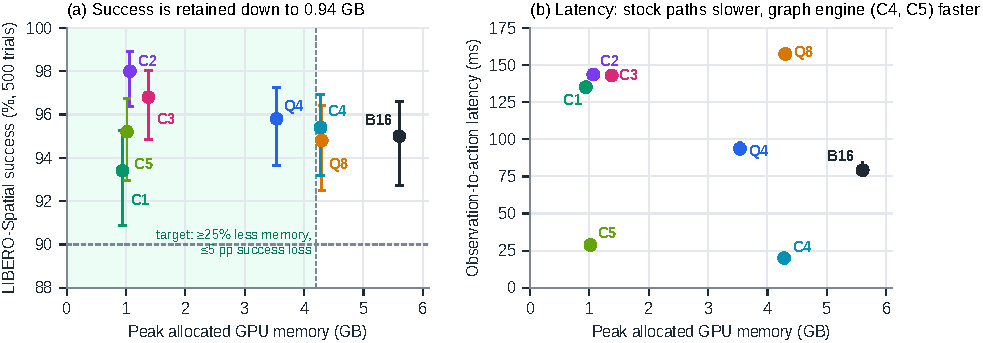
\includegraphics[width=\textwidth]{figures/tradeoff.pdf}
\caption{Reserved-trial trade-offs. (a) Success with 95\% Wilson intervals; the green region meets \h1's memory and success targets. (b) Median latency with p95 tick. Q8/Q4 come from Study A, C1--C4 from Study B (C4 with the graph engine); both B16 controls produce identical outcomes.}
\label{fig:tradeoff}
\end{figure*}

\subsection{Where compression fails (\h2)}
Fig.~\ref{fig:sens} shows 10-trial smoke results; B16 scores 8/10 on the same states. The language decoder is the precision bottleneck. Its best 3-bit and 2-bit variants score 7/10 and 1/10, and 3-bit results vary with the quantization axis (7/10 versus 0/10). Vision blocks and action MLPs keep 8/10 at 2 bits under every tested variant. Structure behaves the same way. Removing 8 of 28 language layers or 50\% of its key--value heads scores 0/10 and 2/10, respectively. Vision keeps 8/10 with 50\% of channels or heads removed and with 8 of 24 layers removed. Action modules degrade gradually. These smoke screens are coarse. At 100 development trials, removing 75\% of action attention heads scores 69/100 and fails the 77/100 gate, although its smoke score was 7/10. Combining individually safe cuts also fails: joint channel and depth reductions score 70/100 and 65/100.

\begin{figure*}[t]
\centering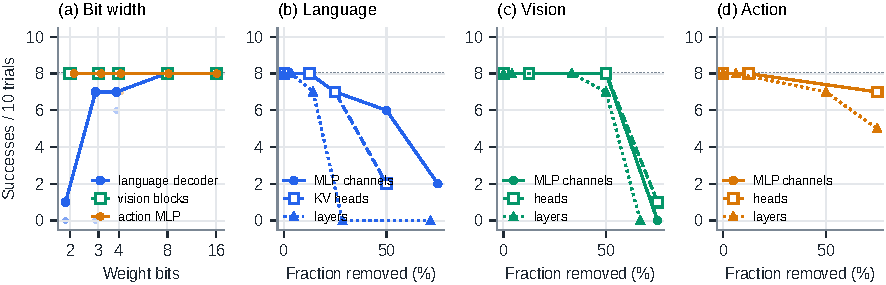
\includegraphics[width=\textwidth]{figures/sensitivity.pdf}
\caption{Module sensitivity (10 trials per point; dotted line: B16 at 8/10). (a) Best tested variant per bit width; faint points show other variants. (b--d) Structured removal by module. Missing points were not tested because adjacent strengths already failed.}
\label{fig:sens}
\end{figure*}

These results guided the joint recipes. C2 keeps NF4 in the language decoder and uses 2-bit HQQ in the vision and action modules: 0.98\,GB of weights and 1.07\,GB peak memory. C1 adds MLP channel removal and reaches the smallest footprint, 0.84\,GB. All four joint recipes pass \h1 by a wide margin on reserved trials (Fig.~\ref{fig:tradeoff}a).

\subsection{Memory is not speed (\h3)}
Under the stock execution path every compressed policy is slower than B16 (Fig.~\ref{fig:tradeoff}b). Q8 doubles latency (1.99$\times$), Q4 costs 1.18$\times$, and C1--C3 cost 1.74--1.85$\times$. The cause is launch overhead, not arithmetic. A profile of one stock prediction (\texttt{launch\_profile.json}) shows B16 launching 4{,}989 kernels with the GPU busy 36\,ms of 79\,ms. Q4 adds a dequantization kernel per linear layer (5{,}576 launches). LLM.int8 launches 9{,}302 kernels and synchronizes with the host 691 times (B16: 118): its 192 \texttt{nonzero} calls (B16: 11) force the host to wait for the GPU.

We therefore wrote a CUDA-graph engine (\texttt{evaluation/fastpath.py}). It precomputes everything that depends only on the instruction, captures one graph per prompt, fuses elementwise kernels with \texttt{torch.compile}, and dequantizes NF4 with one Triton kernel that matches bitsandbytes bit for bit. Table~\ref{tab:ladder} separates its effect from the compression. The engine alone takes B16 from 77.5 to 28.5\,ms. On that fair baseline NF4 weights cost latency: 36.8\,ms with four flow steps against 28.5\,ms, in exchange for 3.8$\times$ less peak memory (1.51 versus 5.70\,GB). Dense bf16 copies of the NF4-rounded weights remove the dequantization (24.7\,ms) at 5.45\,GB. C4 combines NF4 on all modules, an INT8 embedding table, no pruning, no calibration data and one flow step; we chose these to remove task-specific components, not by tuning on outcomes. It runs at 31.6\,ms in 1.51\,GB. The engine captures one graph per instruction; priming ten prompts took 109\,s, which the latencies exclude. \h3 holds for the stock path: memory and latency are independent, and execution sets latency.

\begin{table}[t]
\centering\footnotesize
\caption{Latency attribution (pipeline median, p95 in parentheses; $3\times500$ predictions). Peak is allocated GPU memory. Success: of 500 reserved trials; dashes were not run.}
\label{tab:ladder}
\begin{tabular}{@{}lcccc@{}}
\toprule
Variant & Steps & Median (p95) ms & Peak GB & Success \\
\midrule
B16, stock path & 4 & 77.5 (80.5) & 5.61 & 475 \\
B16, graph engine & 4 & 28.5 (28.9) & 5.70 & 474 \\
B16, graph engine & 1 & 24.8 (25.1) & 5.70 & --- \\
NF4 all, graph, packed & 4 & 36.8 (37.7) & 1.51 & 486 \\
NF4 all, graph, dense & 1 & 24.7 (24.9) & 5.45 & --- \\
NF4 all, graph, packed (C4) & 1 & 31.6 (32.0) & 1.51 & 490 \\
\bottomrule
\end{tabular}
\end{table}

\subsection{Failure analysis (\h4)}
\textbf{Failures are timeouts in one task.} Rollouts are deterministic given state and seed: the two B16 runs agree on all 500 episodes. All 25 B16 failures hit the 280-step limit; none crashed. Seventeen occur in task~5, ``pick up the black bowl on the ramekin'' (Fig.~\ref{fig:tasks}). Quantization mostly inherits these failures: 22 of Q8's 26 and 17 of Q4's 21 failed states also fail under B16.

\textbf{Task 5 decides the aggregate.} C2's net gain of 15 successes comes entirely from task~5 (33$\rightarrow$48/50); changes in the other nine tasks cancel out. C1 loses 4 of its net 8 in task~5. A task where small action perturbations flip outcomes can create apparent ``improvements'' from compression. C2's $+3.0$-point gain is therefore not evidence that 2-bit weights improve the policy.

C4 shows the same pattern: 11 of its net 15 successes come from task~5 (33$\rightarrow$44/50), and four more from three other tasks. Two controls locate the effect (Table~\ref{tab:ladder}). B16 through the graph engine scores 474/500 ($-0.2$ points, 95\% CI $-1.2$ to $+0.8$), so the engine does not change success. The same NF4 weights with four flow steps score 486/500 ($+2.2$, $+0.8$ to $+3.8$), and one step adds four successes, within noise. The gain therefore appears with quantized weights, not with the engine or the solver. We report it as unexplained and make no claim that quantization improves the policy.

\begin{figure}[t]
\centering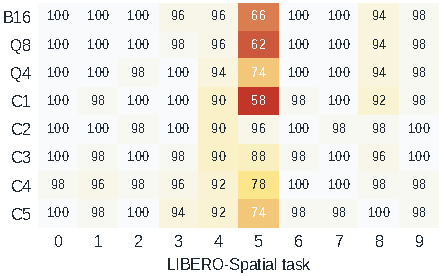
\includegraphics[width=\columnwidth]{figures/tasks.pdf}
\caption{Per-task success (\%, 50 reserved trials per cell). Task 5 accounts for most failures and most differences between arms.}
\label{fig:tasks}
\end{figure}

\begin{figure}[t]
\centering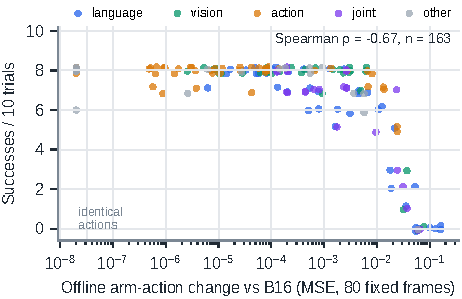
\includegraphics[width=\columnwidth]{figures/divergence.pdf}
\caption{Offline action change on 80 fixed development frames versus 10-trial success, for 163 recipes (jittered vertically). Recipes with identical actions sit at the left edge.}
\label{fig:div}
\end{figure}

\textbf{Offline divergence screens, but does not rank.} For each recipe we measured the mean squared change in physical arm commands against B16 on 80 fixed frames, which needs no simulator. Across 163 recipes it correlates with smoke success ($\rho=-0.67$, $p<10^{-21}$; Fig.~\ref{fig:div}). Below $10^{-4}$, 64 of 65 recipes score $\geq$7/10; above $10^{-3}$, only 30 of 62 do. Among the 24 recipes that reached development trials, the correlation is weak and not significant ($\rho=-0.27$, $p=0.21$). \h4 holds for screening but not for ranking: closed-loop trials remain necessary among near-lossless recipes.

\subsection{Negative result: smaller backbone}
We replaced Qwen with SmolVLM2-500M~\cite{smolvlm} plus a trained adapter and fine-tuned the adapter, action head and predictor for 10{,}000 steps. It reached 2.2\% on reserved trials and was 16$\times$ slower than B16, because SmolVLM tiles each image into 17 crops of 512 pixels. A later study fixed an image-scaling bug and adapted all decoder layers. It reached 31/100 development successes against 82/100 for B16. Within our budget, compressing the trained policy beats replacing its backbone.

\section{Recommendations}
\begin{enumerate}
\item \textbf{For a single-GPU deployment with a memory limit, start with Q4.} It uses a standard bitsandbytes configuration, saves 37\% of peak memory, shows no detectable success loss, and costs 18\% latency on the stock path.
\item \textbf{For latency, run a CUDA-graph engine.} It makes B16 itself 2.7$\times$ faster (28.5\,ms). C4 runs at 31.6\,ms in 1.51\,GB; B16 with one flow step runs at 24.8\,ms in 5.7\,GB.
\item \textbf{Below 1.6\,GB, use C3 or C4.} Both keep the full vocabulary and use no calibration data. C1 and C2 are smaller but accept only the 53 token IDs in the LIBERO prompts.
\item \textbf{Avoid LLM.int8 at batch size one.} It is slower than NF4 and saves less memory.
\item \textbf{Spend precision on the language decoder}, and compress vision and action modules first.
\item \textbf{Screen with offline action change, confirm with $\geq$500 paired trials.} Ten or even 100 trials cannot rank near-lossless recipes, and per-task paired transitions expose single-task effects such as task~5.
\end{enumerate}

\section{Limitations and Conclusion}
We evaluated one suite (LIBERO-Spatial), one checkpoint, one GPU and one seed per state. Success on Object, Goal or Long suites, on other hardware, and on a real robot is untested. Development and smoke selection used 10--100 trials, so sensitivity curves are coarse. C1 and C2 depend on the test prompts' vocabulary, and C1's pruning on development observations of the same tasks; C3 and C4 use neither. We chose every arm on smoke and development states, never on reserved trials, but the same 500 reserved states score all arms with no multiple-comparison correction. The graph engine assumes one observation, two equal-size images and unpadded prompts per call, and its fused kernels change bf16 rounding, so we measured success through the engine. Compressed archives are rebuilt from the original checkpoint plus a recipe and are not standalone Hugging Face checkpoints.

Post-training compression is effective for VLA-JEPA. NF4 decoder quantization meets our memory and success targets. Joint recipes keep $\geq$93\% success in under 1.6\,GB, a 3.5--6$\times$ reduction. The language decoder limits further compression, and a single hard task drives most differences between arms. Latency rises under the stock path; a graph engine removes the overhead for every variant, and C4 runs at 31.6\,ms in 1.51\,GB. Fused 4-bit GEMM kernels and evaluation on longer-horizon suites are the next steps.

\bibliographystyle{IEEEtran}
\bibliography{refs}
\end{document}
